\documentclass{article}

\usepackage{graphicx}
\usepackage{tikz}
\usepackage{tikzsymbols}
\usetikzlibrary{calc,patterns,shapes.geometric}
\pagestyle{empty}
\usepackage[margin=0pt]{geometry}
\geometry{papersize={14in,12in}}

\def\centerarc[#1](#2)(#3:#4:#5){\draw[#1] ($(#2)+({#5*cos(#3)},{#5*sin(#3)})$) arc (#3:#4:#5);}

\begin{document}
	\begin{figure}
		\centering
		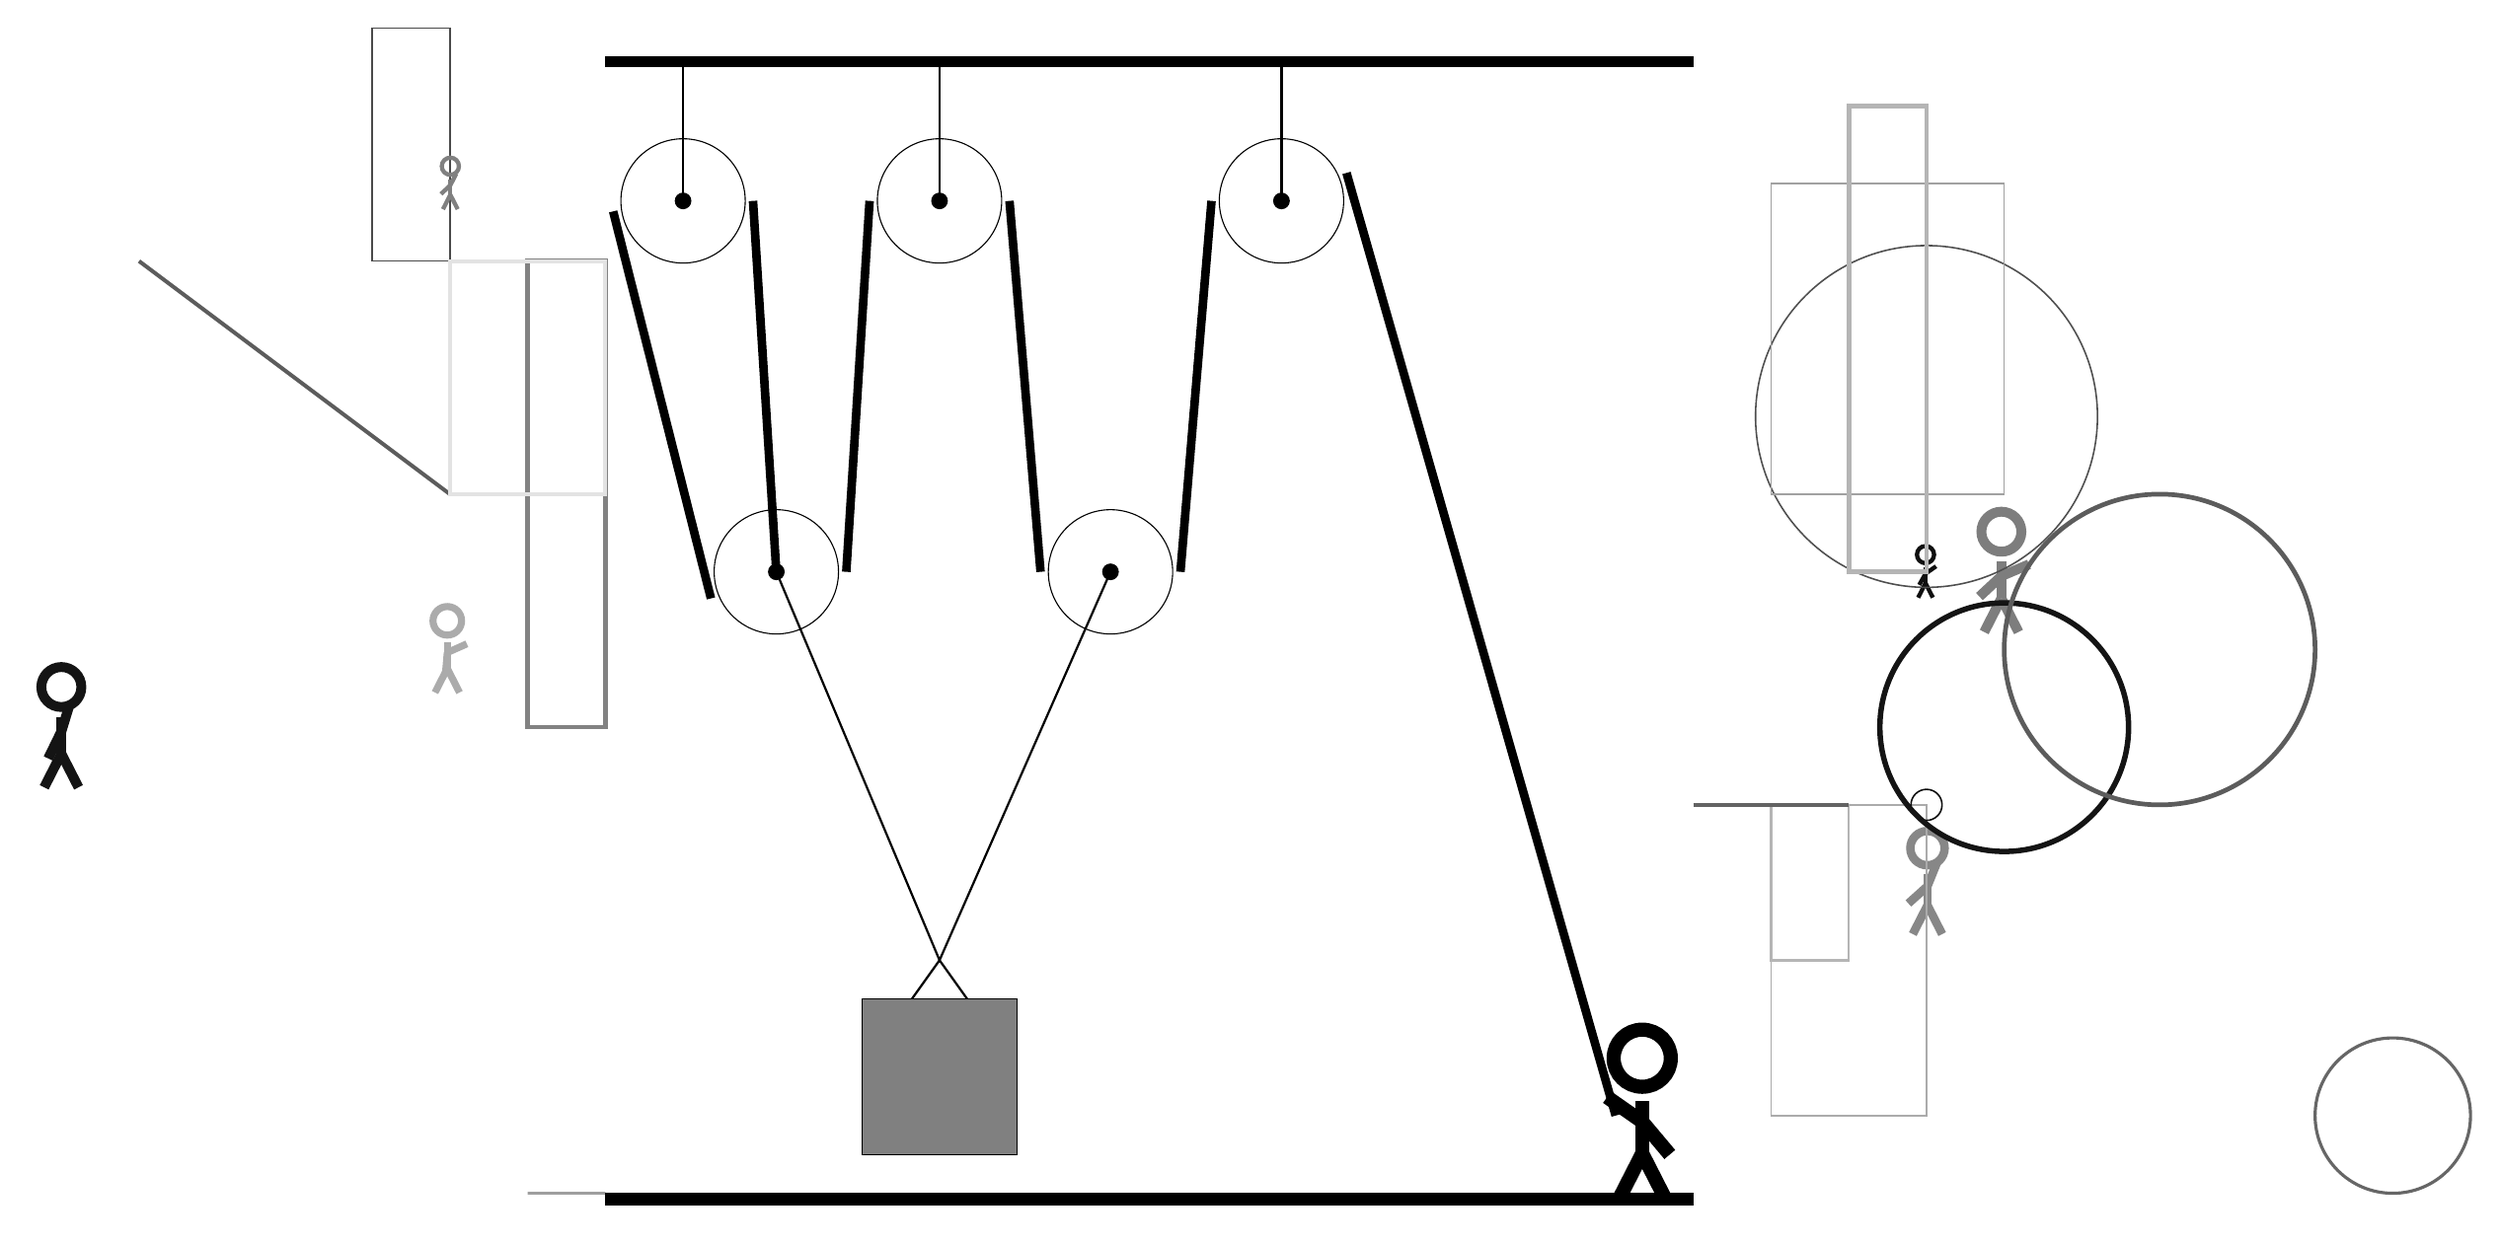
\begin{tikzpicture}
			%%%%% START %%%%%
			
			\draw[fill=black] (-2, 11.5) rectangle (12, 11.625);
			
			\draw (-1, 9.775) circle (0.8);
			\draw[fill=black] (-1, 9.775) circle (0.1);
			\draw[thick] (-1, 9.775) -- (-1, 11.5);
			
			\draw (2.3, 9.775) circle (0.8);
			\draw[fill=black] (2.3, 9.775) circle (0.1);
			\draw[thick] (2.3, 9.775) -- (2.3, 11.5);
			
			\draw (6.7, 9.775) circle (0.8);
			\draw[fill=black] (6.7, 9.775) circle (0.1);
			\draw[thick] (6.7, 9.775) -- (6.7, 11.5);
			
			\node[line width=0.2mm, color=black!47] at (15, 1) {\Strichmaxerl[6][42][68]};
			
			\draw[line width=0.2mm, color=black!33] (13, 2) rectangle (15, -2);
			\node[line width=0.3mm, color=black!51] at (16, 5) {\Strichmaxerl[7][43][23]};
			\draw [line width=0.4mm, color=black!60](21, -2) circle (1.0);
			\draw[line width=0.2mm, color=black!91] (-3, 6) rectangle (-3, 3);
			\draw[line width=0.5mm, color=black!64](-4, 6) -- (-8, 9);
			
			\draw [line width=0.2mm, color=black!95](15, 2) circle (0.2);
			\node[line width=0.7mm, color=black!94] at (15, 5) {\Strichmaxerl[3][61][35]};
			\node[line width=0.4mm, color=black!92] at (-9, 3) {\Strichmaxerl[7][64][73]};
			
			\draw [line width=0.2mm, color=black!69](15, 7) circle (2.2);
			\draw [line width=0.7mm, color=black!92](16, 3) circle (1.6);
			
			\draw[line width=0.6mm, color=black!49] (-3, 9) rectangle (-2, 3);
			\draw[line width=0.2mm, color=black!71] (-4, 9) rectangle (-5, 12);
			
			\draw[line width=0.5mm, color=black!11] (-4, 9) rectangle (-2, 6);
			\draw[line width=0.4mm, color=black!38] (-3, -3) rectangle (-2, -3);
			\node[line width=0.7mm, color=black!50] at (-4, 10) {\Strichmaxerl[3][43][63]};
			\draw[line width=0.2mm, color=black!37] (13, 10) rectangle (16, 6);
			
			\draw [line width=0.6mm, color=black!64](18, 4) circle (2.0);
			\draw[line width=0.3mm, color=black!29] (13, 0) rectangle (14, 2);
			
			\draw[line width=0.5mm, color=black!61](12, 2) -- (14, 2);
			\draw[line width=0.6mm, color=black!29] (14, 11) rectangle (15, 5);
			
			\node[line width=0.5mm, color=black!33] at (-4, 4) {\Strichmaxerl[5][85][24]};
			
			\draw (0.2, 5) circle (0.8);
			\draw[fill=black] (0.2, 5) circle (0.1);
			
			\draw (4.5, 5) circle (0.8);
			\draw[fill=black] (4.5, 5) circle (0.1);
			
			\draw[thick] (0.2, 5) -- (2.3, 0)  -- (4.5, 5);
			\draw[thick]  (1.8, -0.7) -- (2.3, 0) -- (2.8, -0.7);
			\draw[fill=black!50] (1.3, -0.5) rectangle (3.3, -2.5);
			
			\draw[line width=1.1mm] (0.2, 5) -- (-0.1, 9.775);
			\centerarc[line width=1.1mm](-1, 9.775)(0:200:0.9);
			\draw[line width=1.1mm] (-1.9, 9.64) -- (-0.6415, 4.658);
			\centerarc[line width=1.1mm](0.2, 5)(200:360:0.9);
			\draw[line width=1.1mm](1.1, 5) -- (1.4, 9.775);
			\centerarc[line width=1.1mm](2.3, 9.775)(0:180:0.9);
			\draw[line width=1.1mm] (3.2, 9.775) -- (3.6, 5);
			\centerarc[line width=1.1mm](4.5, 5)(180:360:0.9);
			\draw[line width=1.1mm] (5.4, 5) -- (5.8, 9.775);
			\centerarc[line width=1.1mm](6.7, 9.775)(20:180:0.9);
			\draw[line width=1.1mm](7.537, 10.135)  -- (11, -2);
			
			\node at (11.3, -2) {\Strichmaxerl[10][-35][-50]};
			
			\draw[fill=black] (-2, -3) rectangle (12, -3.15);
			
			%%%%% END %%%%%
		\end{tikzpicture}
	\end{figure}	
\end{document}